\chapter{Results}

\section{HRV cloud objects}
The derivation of cloud objects as described in Sec. \ref{sec:cloud} yielded a total of \num{17301} HRV cloud objects for the five case days with \SI{84}{\percent} single cell objects and \SI{16}{\percent} complex objects, which are multi cell objects with a number of splits and merges. The vast majority of the single cell objects has only a rather short life time of \SIrange{15}{30}{\minute} with a median life time of \SI{30}{\minute} (Fig.~\ref{fig:cell_ltime}). As it can been seen in Fig.~ \ref{fig:cell_ltime} the life time distribution of the complex objects is broader then the one of the single cells. As to be expected, the complex objects also have longer life time with a median of \SI{60}{\minute}. There are no complex objects with a life time of lower than \SI{30}{\minute}. This is due to the definition of the complex objects. There are at least two time steps needed to develop splits or merges, so that the minimum life time of these objects is at least \SI{30}{\minute}. The multi cell objects can be quite complex with up to \num{26} splits or merges in one object (Fig.~\ref{fig:splits_merges}). Those objects represent large compact cloud fields which usually are present for a longer time range. But most complex objects have only have very few splits or merges with median value of one split or merge. These objects represent smaller cloud objects which grow together to form larger objects. On contrary, splits are roughly \num{1.3} times more frequent in the objects than merges and every object has at least one split whereas there are objects which have no merge. One reason for this is, that the rather large and long living cloud fields tend dissolve on the boundaries and so create smaller objects that not merge again.

Separating the complex objects at the split and merge points, and only conserving the objects prior to these points, an additional number of a bit over \num{5000} single cells can be derived. The life time distribution of the single objects derived from the complex objects is quite similar to the distribution of the single cell objects (Fig.~\ref{fig:single_cell}).

When only taking into account all single cells with a life time of at least \SI{30}{\minute}, to be consistent with the ground truth definition, the number of eligible objects decreases to almost \num{6200} objects. But, as not all the validation area is covered by the radars, only the objects inside the radar covered area can be used for the validation. this reduces the number of eligible objects to 5880. The further analysis was conducted with these objects.

\begin{figure}[htbp]
\centering
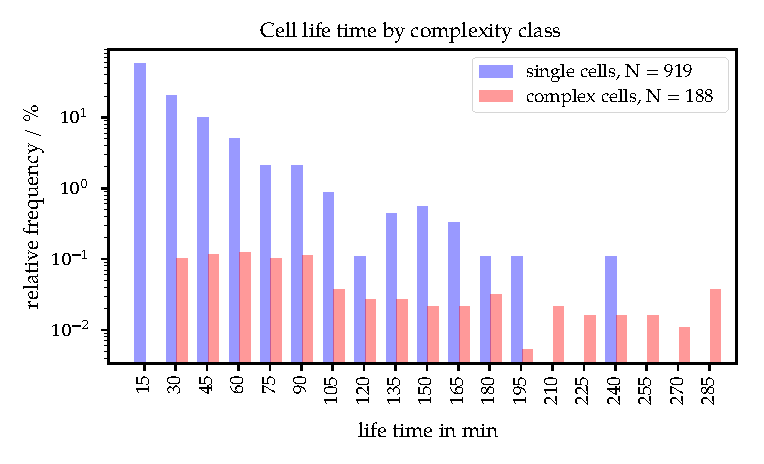
\includegraphics[width=\textwidth]{/home/lenk/Tropos/VSA_NWCSAF/Grafiken/Abbildungen/cellclass_lifetime.pdf}
\caption{Comparison of the life time of single (blue) and multi cell (complex) objects (red).}
\label{fig:cell_ltime}
\end{figure}

\begin{figure}[htbp]
\centering
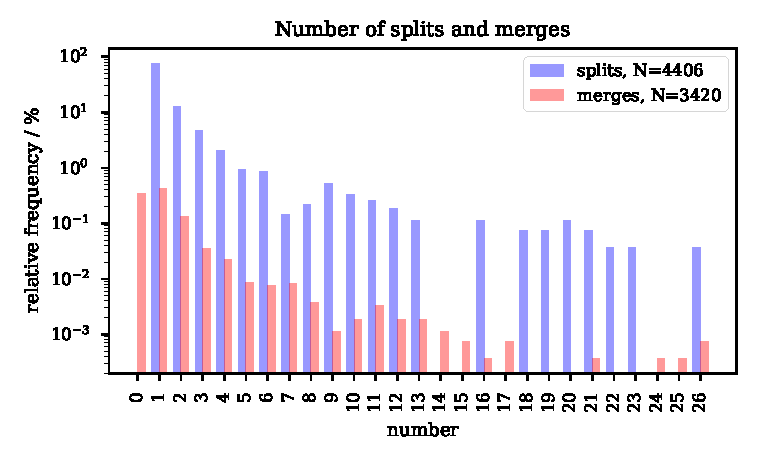
\includegraphics[width=\textwidth]{/home/lenk/Tropos/VSA_NWCSAF/Grafiken/Abbildungen/splits_merges.pdf}
\caption{Distribution of number of splits and merges in the complex objects.}
\label{fig:splits_merges}
\end{figure}

\begin{figure}[htbp]
\centering
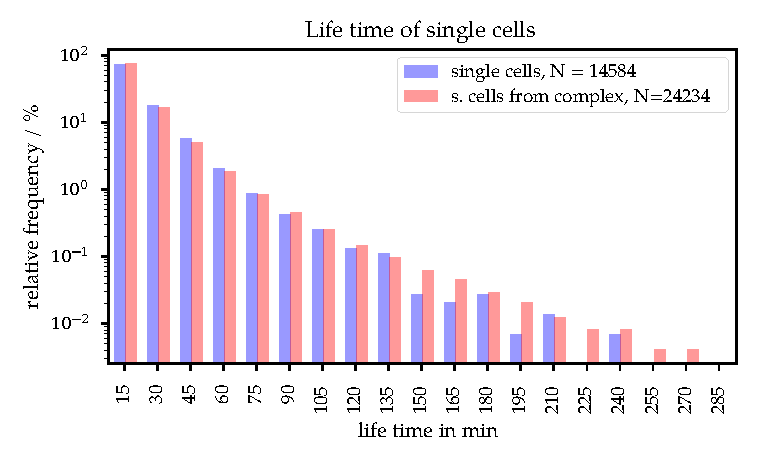
\includegraphics[width=\textwidth]{/home/lenk/Tropos/VSA_NWCSAF/Grafiken/Abbildungen/single_from_complex_lifetime.pdf}
\caption{Comparison of the life time of single cell objects (blue) and the single cell objects derived from complex objects (red).}
\label{fig:single_cell}
\end{figure}

\section{Radar objects}
Using the weather radar data and applying the approach presented in Sec. \ref{sec:haci}, \num{2563} radar objects with a minimum life time of \SI{30}{\minute} could be derived. This is only around \SI{40}{\percent} of the number of cloud objects

\section{Validation results}



